
\newpage
\subsection{Codifica del Prodotto} 

\subsubsection{Analisi statica e automatizzata dei documenti}\label{resocontoProgettazioneArchitetturale}
Tutta la documentazione prodotta in ingresso alla Revisione di Accettazione è stata sottoposta ad una meticolosa attività di verifica
basata su quanto previsto all'interno del documento delle \dext{NormeDiProgetto\_4.0.0}.
Questa attività è stata espletata dai verificatori.
Come avvenuto per la Revisione di Progettazione tutta la documentazione è stata sottoposta ad analisi automatizzata.
La correttezza ortografica si è mantenuta stabile sul valore nullo.

Considerato che i documenti \dext{Manuale Manutentore\_1.0.0} e  \dext{Manuale Utente\_1.0.0} sono redatti in lingua inglese
non è possibile fornire un valore connesso alla metrica \textit{Indice di Gulpease}, in quanto tale metrica è riservata a contenuti 
testuali in lingua italiana.


\begin{center}
    \begin{figure}[!htb]
        \centering
        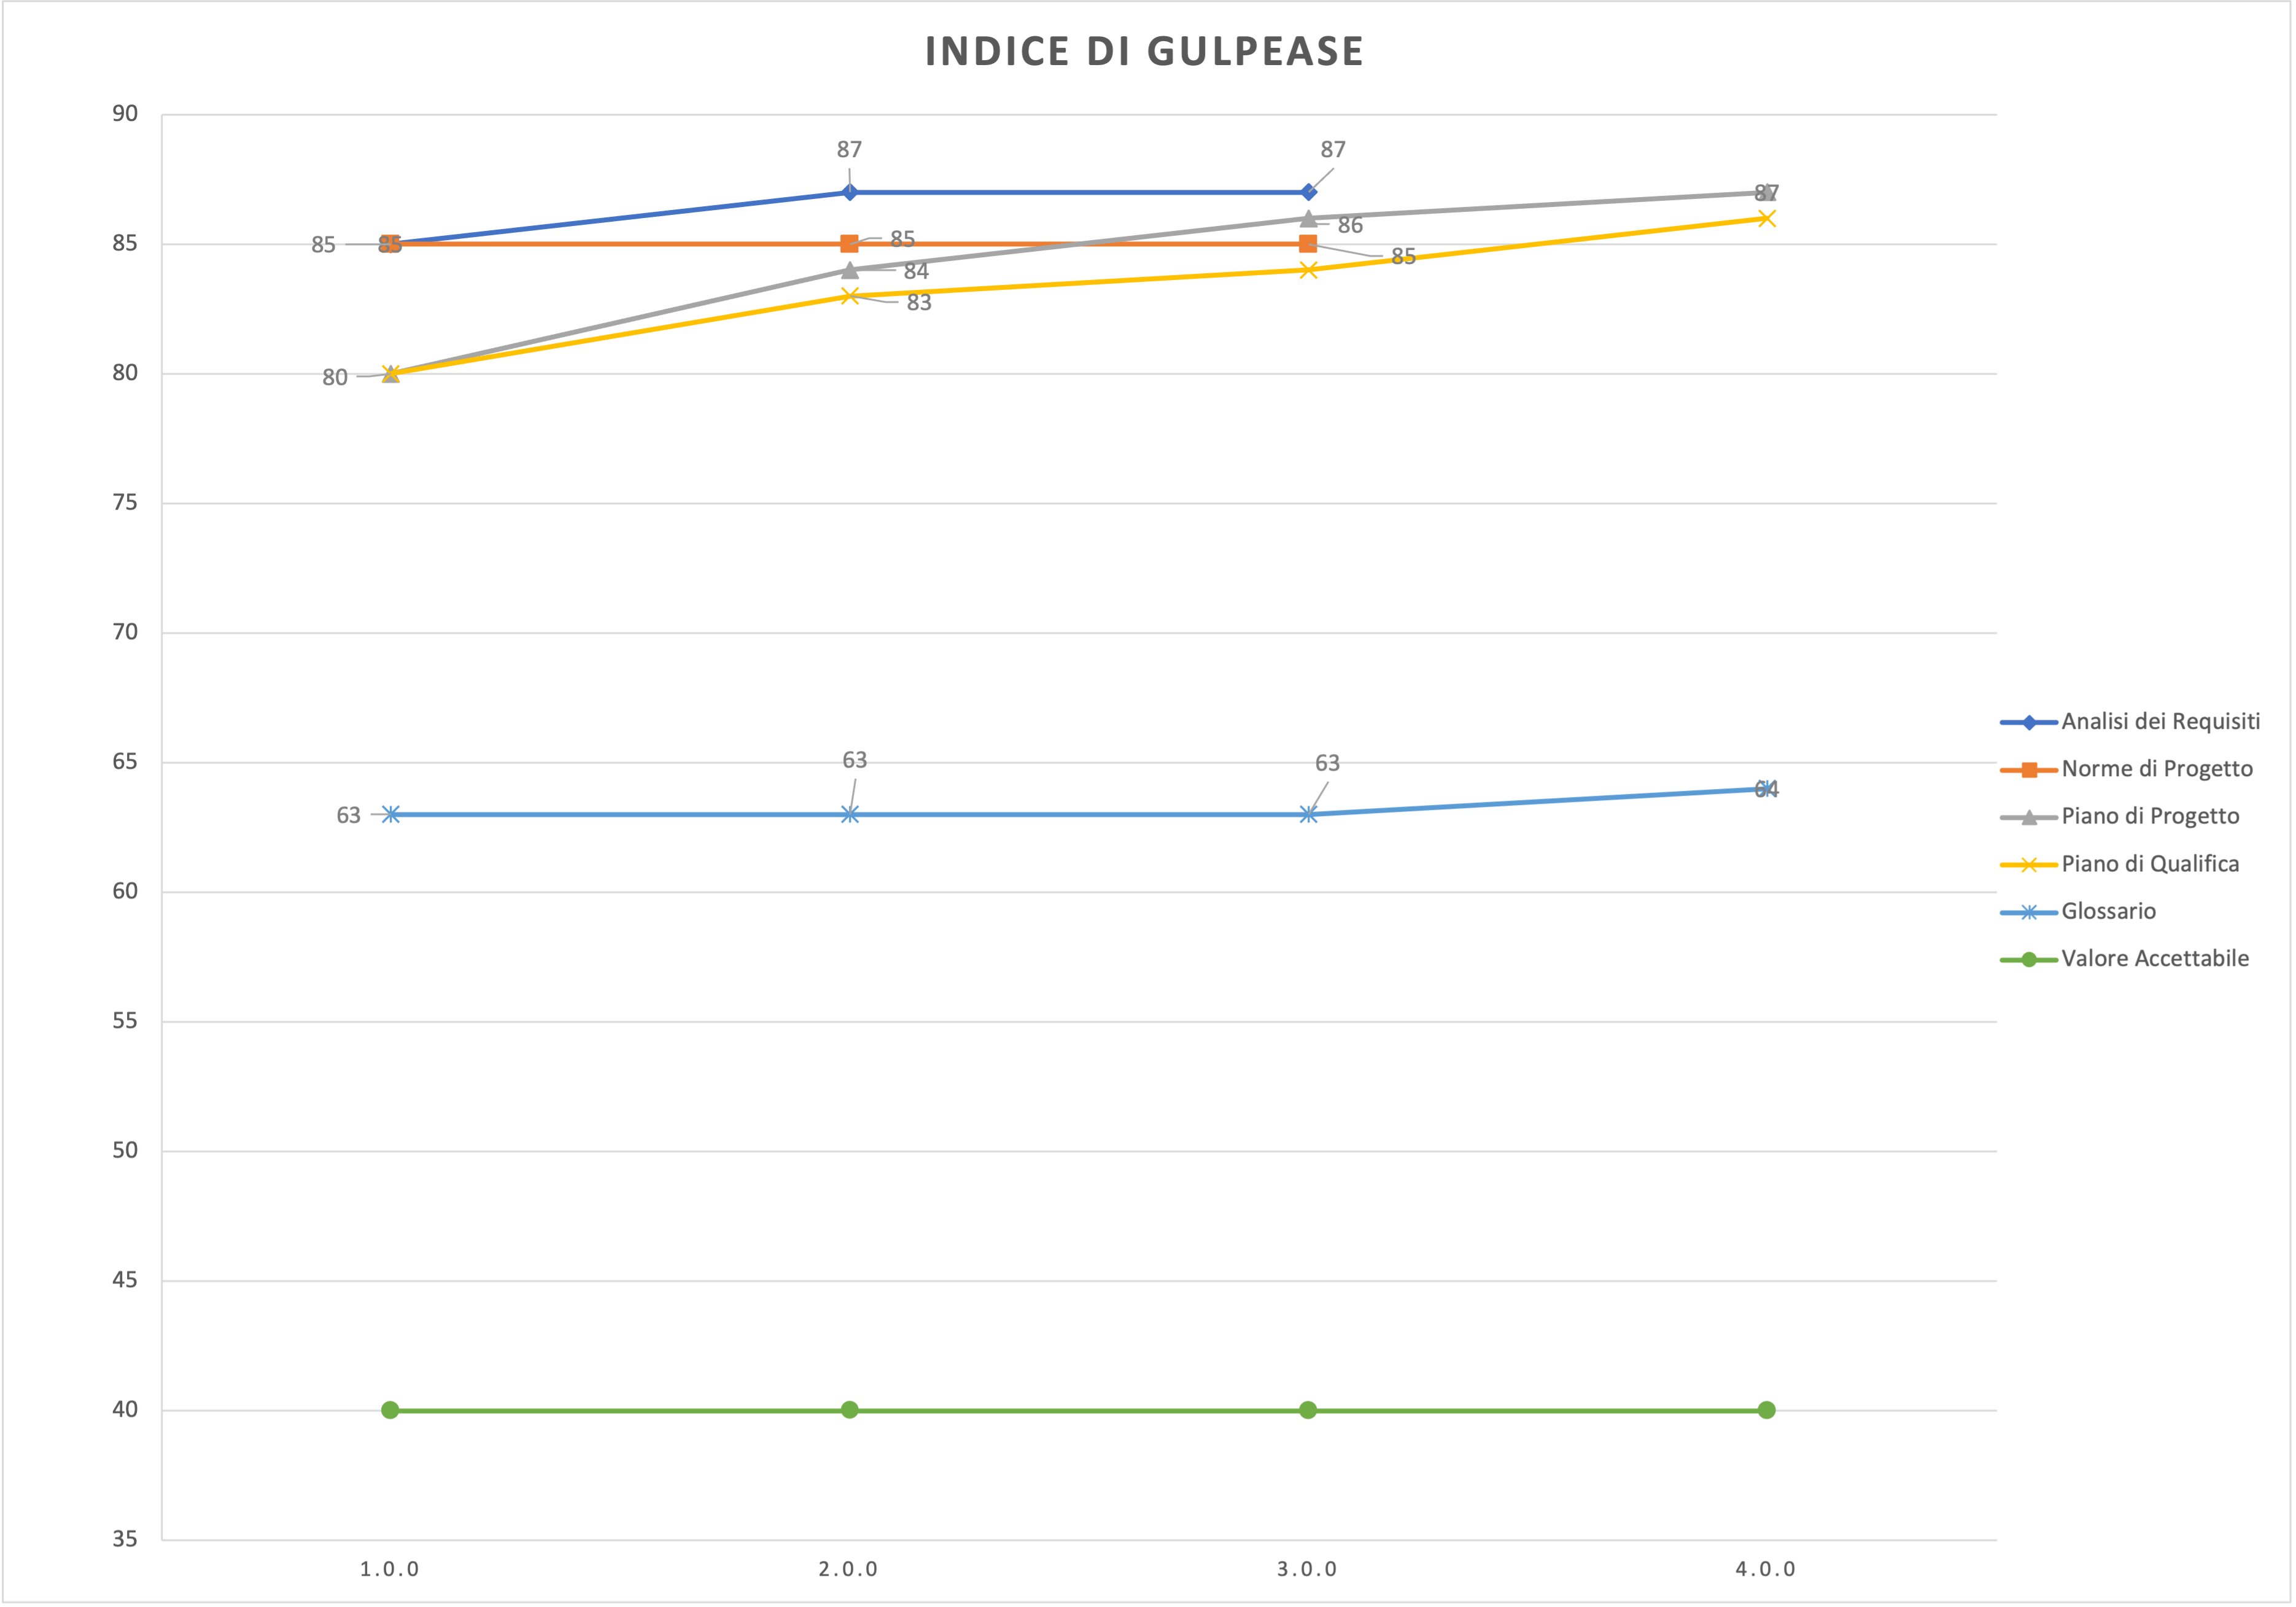
\includegraphics[scale=0.60]{res/images/ra/ra_gulpease.png}
        \caption{Grafico Indice di Gulpease}
    \end{figure}
    \begin{center}
        \rowcolors{2}{white}{blue!20}
        \begin{longtable}{|c|c|}
            \hline
            \rowcolor{lighter-grayer}
            \textbf{Documento}         & \textbf{Indice di Gulpease} \\
            \hline
            \endfirsthead

            \hline
            Verbale Interno 2021-03-10 & 60                          \\
            Verbale Esterno 2021-03-17 & 63                          \\      
            Verbale Interno 2021-03-19 & 63                          \\ 
            
            \hline
            \rowcolor{white}
            \caption{Indice di Gulpease dei verbali}
        \end{longtable}
    \end{center}
\end{center}

\subsubsection{Dettaglio delle verifiche di prodotto}

Così come previsto nelle \dext{Norme di Progetto\_4.0.0} il codice prodotto sino ad ora è stato sottoposto ad un processo di verifica il quale 
ha sfruttato strumenti software atti all'espletamento automatico delle operazioni di accertamento della conformità alle norme previste, nonchè
al rispetto dei valori massimi accettabili dalle singole metriche.
Al fine di rendere più fruibili al lettore i risultati ottenuti all'esito dell'esecuzione delle attività di verifica è stato scelto di presentarli
separatamente per il frontend e per i singoli micro-servizi implementati.

\begin{center}
    \textbf{MPD-S1 COCI} \\
    Grafo relativo ai valori della metrica relativa alla complessità ciclomatica, i risultati si intendono espressi come media dei singoli
    micro servizi.
    \begin{figure}[!htb]
        \centering
        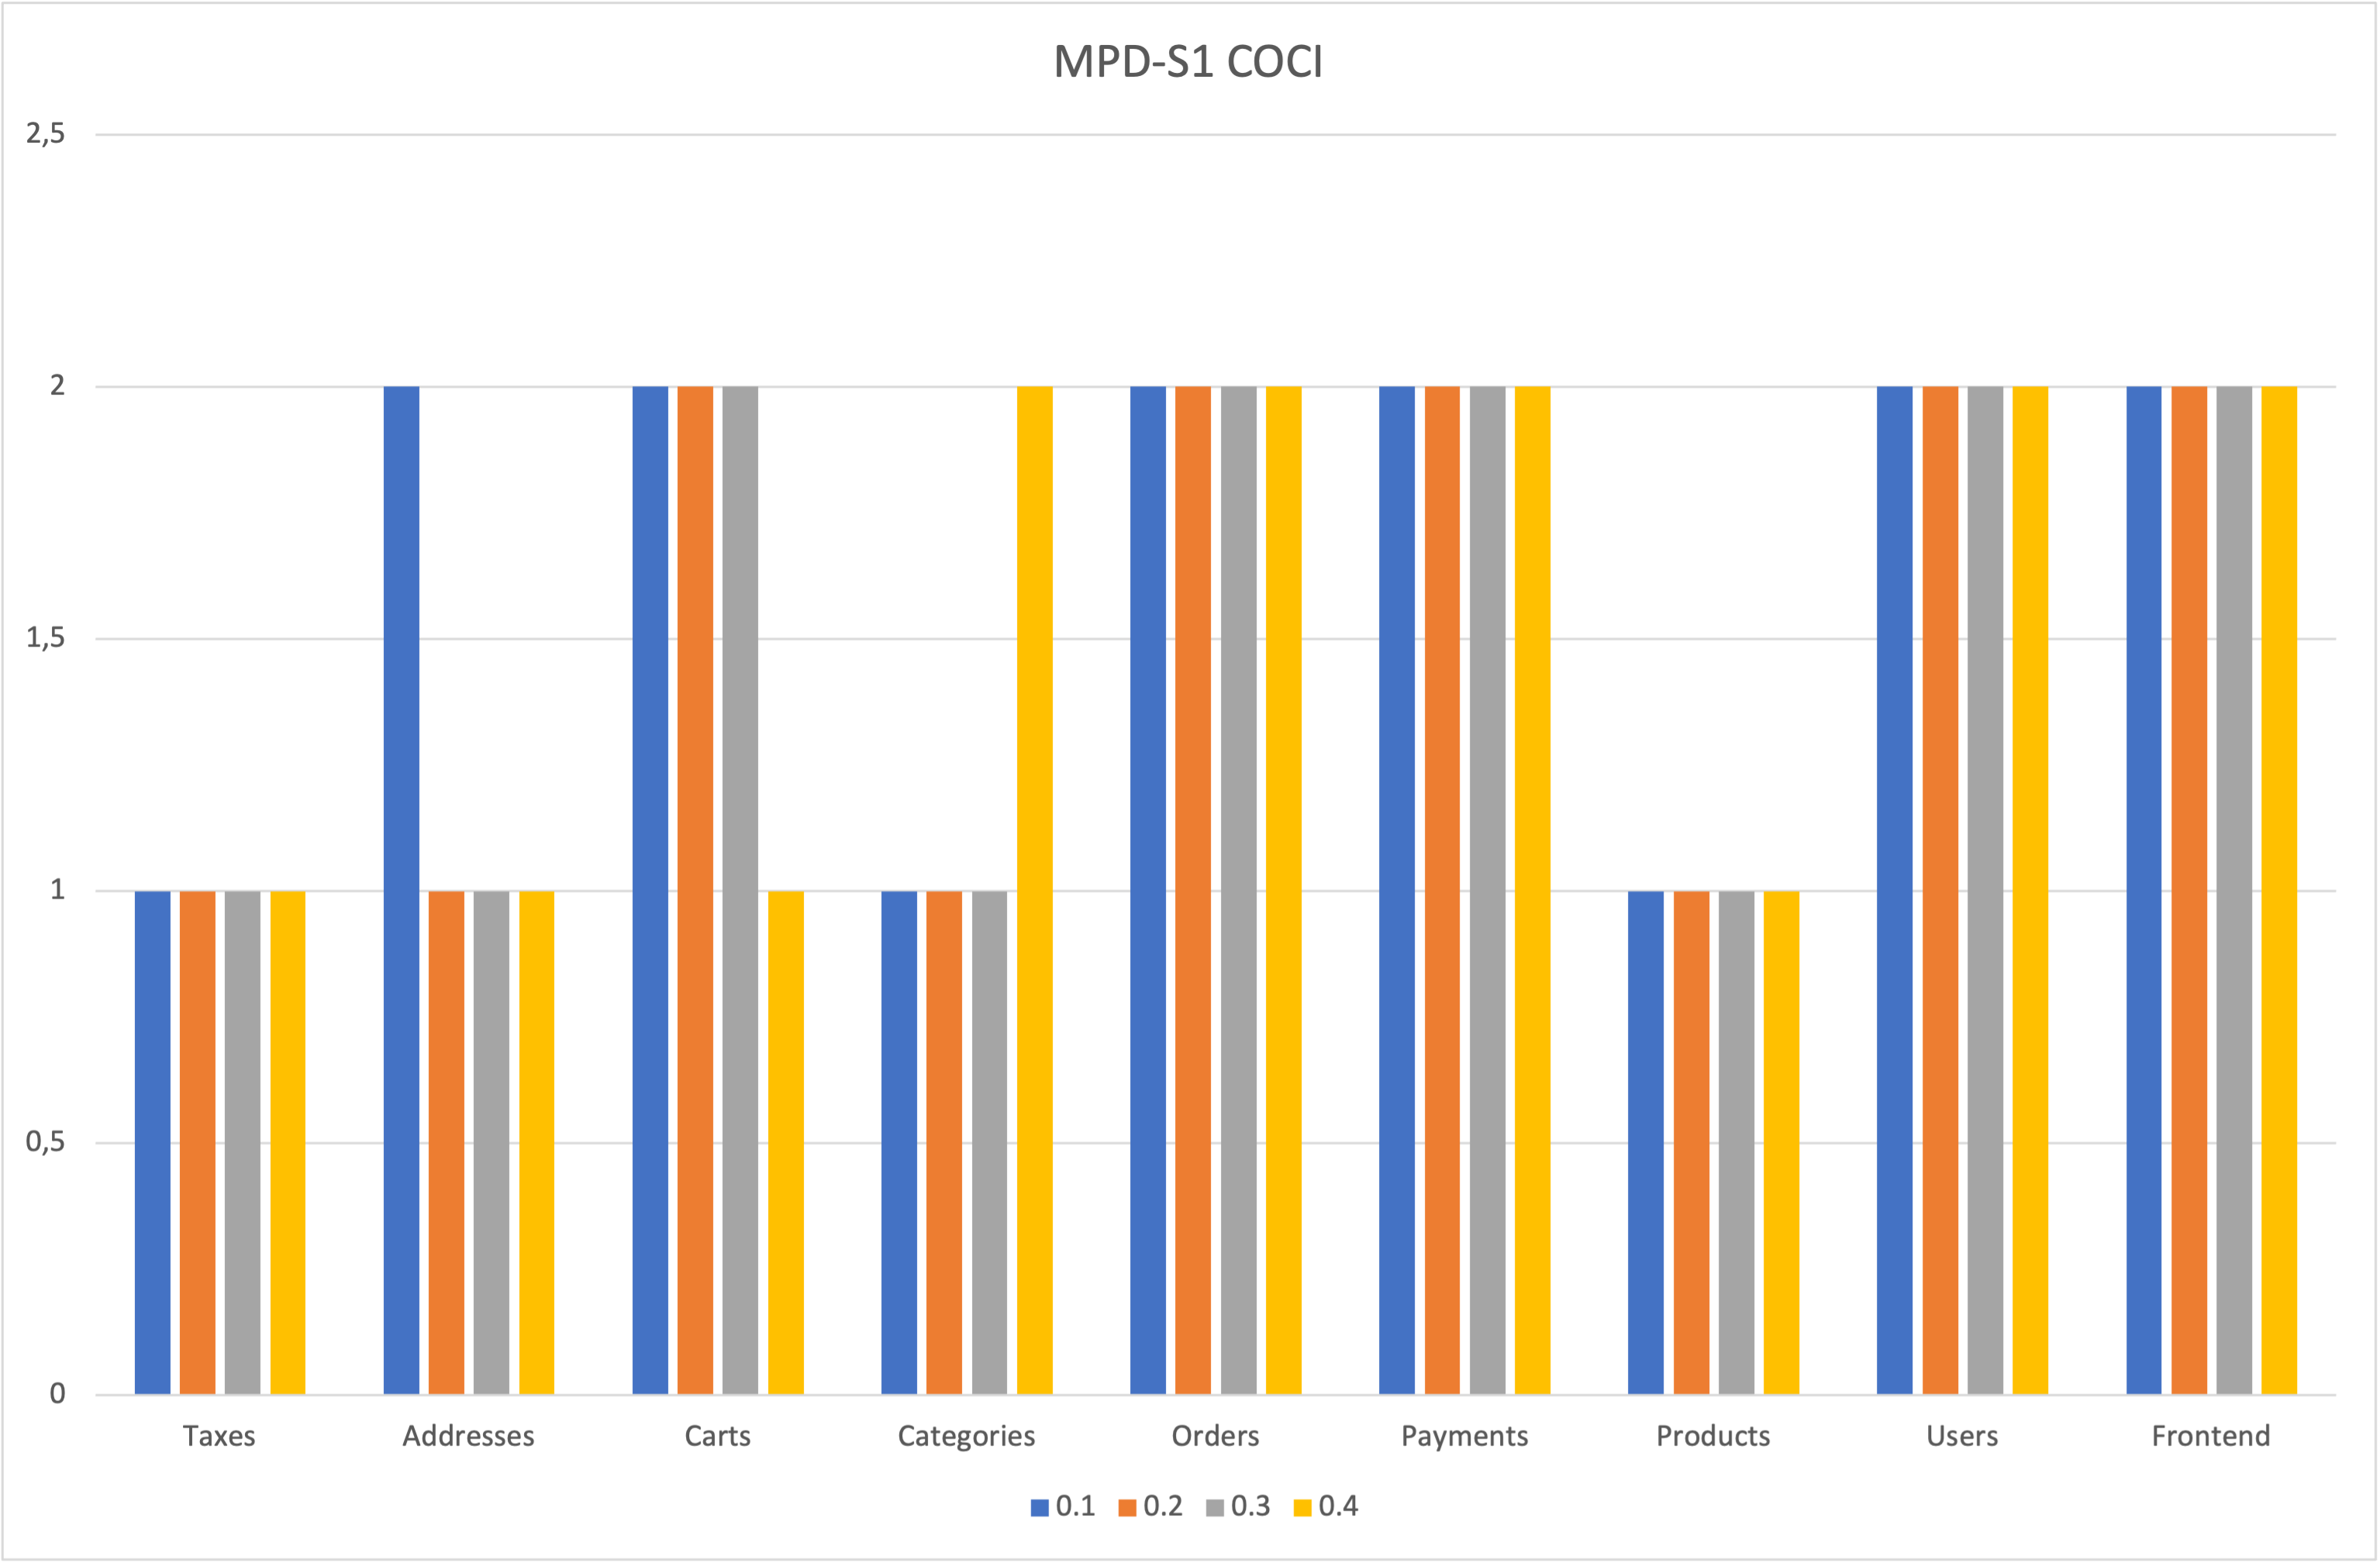
\includegraphics[scale=0.50]{res/images/ra/ra_coci.png}
        \caption{Grafico metrica MPD-S1 COCI | Complessità ciclomatica}
    \end{figure}
    \begin{center}
        \rowcolors{2}{white}{blue!20}
        
    \end{center}
\end{center}

\newpage

\begin{center}
    \textbf{MPD-S2 COEB} \\
    Grafo relativo ai valori della metrica relativa alla complessità delle espressioni booleane, valore desiderabile atteso è 1
    \begin{figure}[!htb]
        \centering
        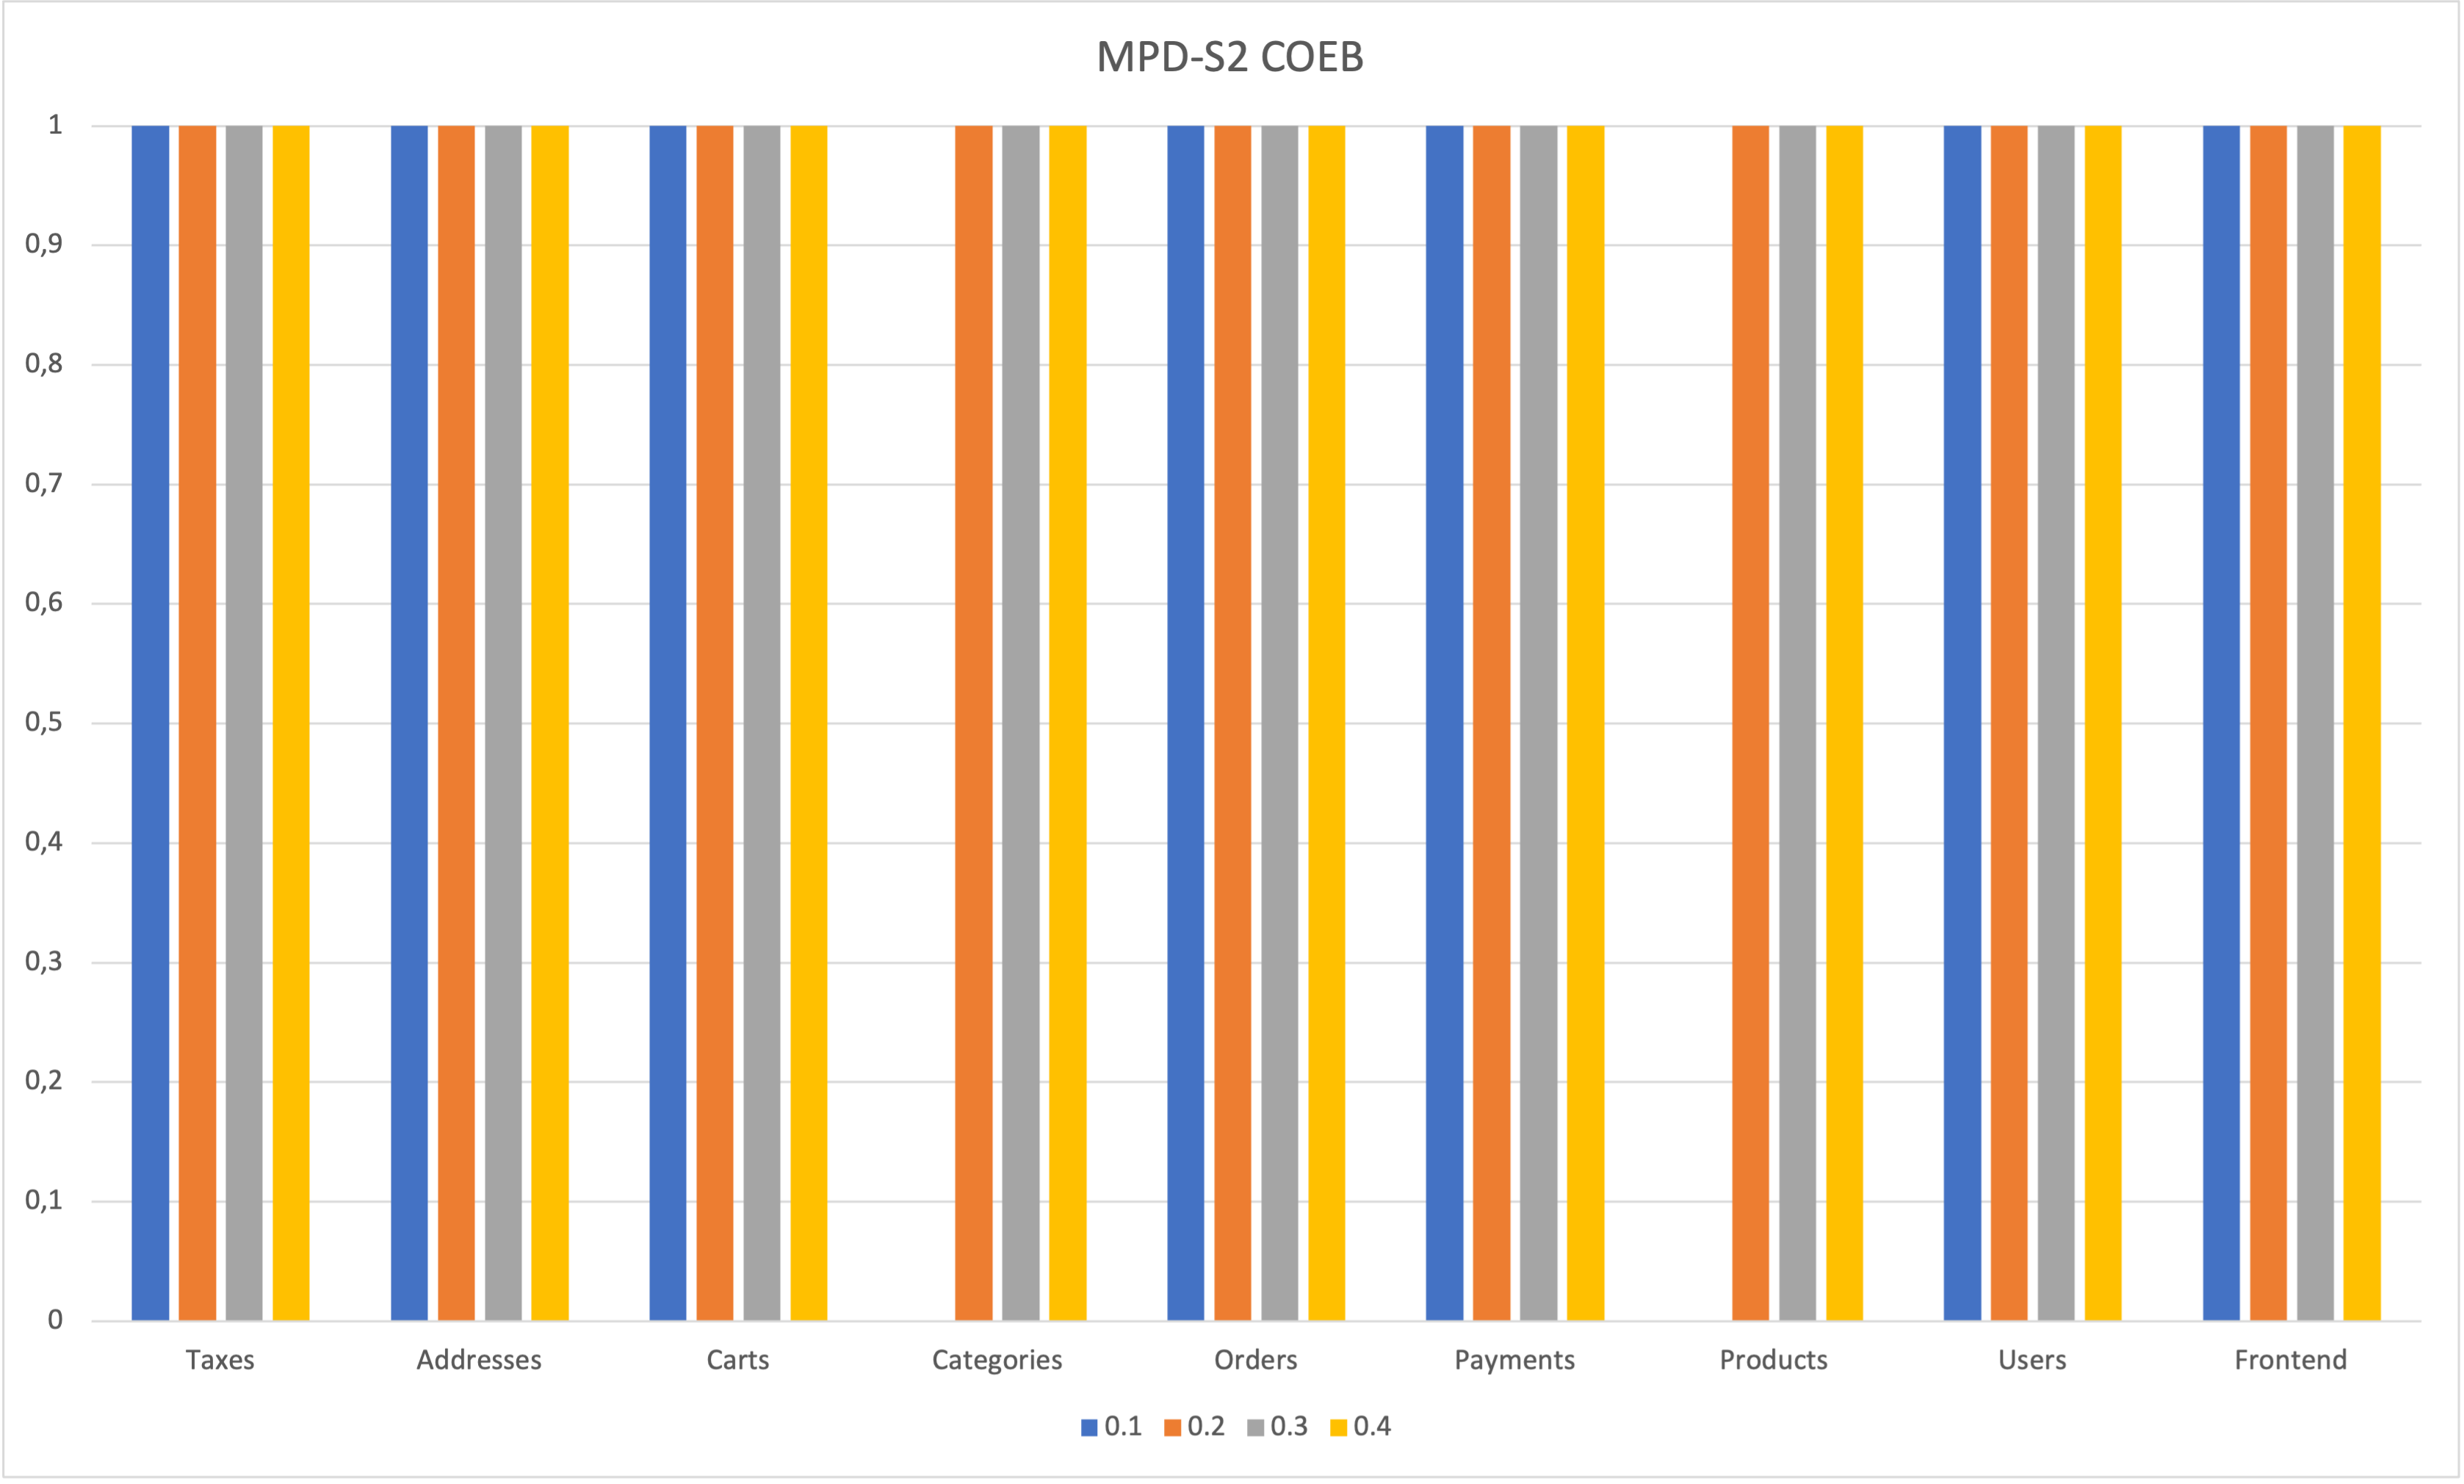
\includegraphics[scale=0.50]{res/images/ra/ra_coeb.png}
        \caption{Grafico metrica MPD-S2 COEB}
    \end{figure}
    \begin{center}
        \rowcolors{2}{white}{blue!20}
    \end{center}
\end{center}

\begin{center}
    \textbf{MPD-S3 LRC} \\
    Grafo relativo ai valori della metrica relativa alla lunghezza delle righe di codice, il grafo rappresenta con il valore 1 i micro-servizi
    che rispettano quanto previsto nelle \dext{NormeDiProgetto\_4.0.0}, ovvero quando la lunghezza massima delle righe è pari a 100     \begin{figure}[!htb]
        \centering
        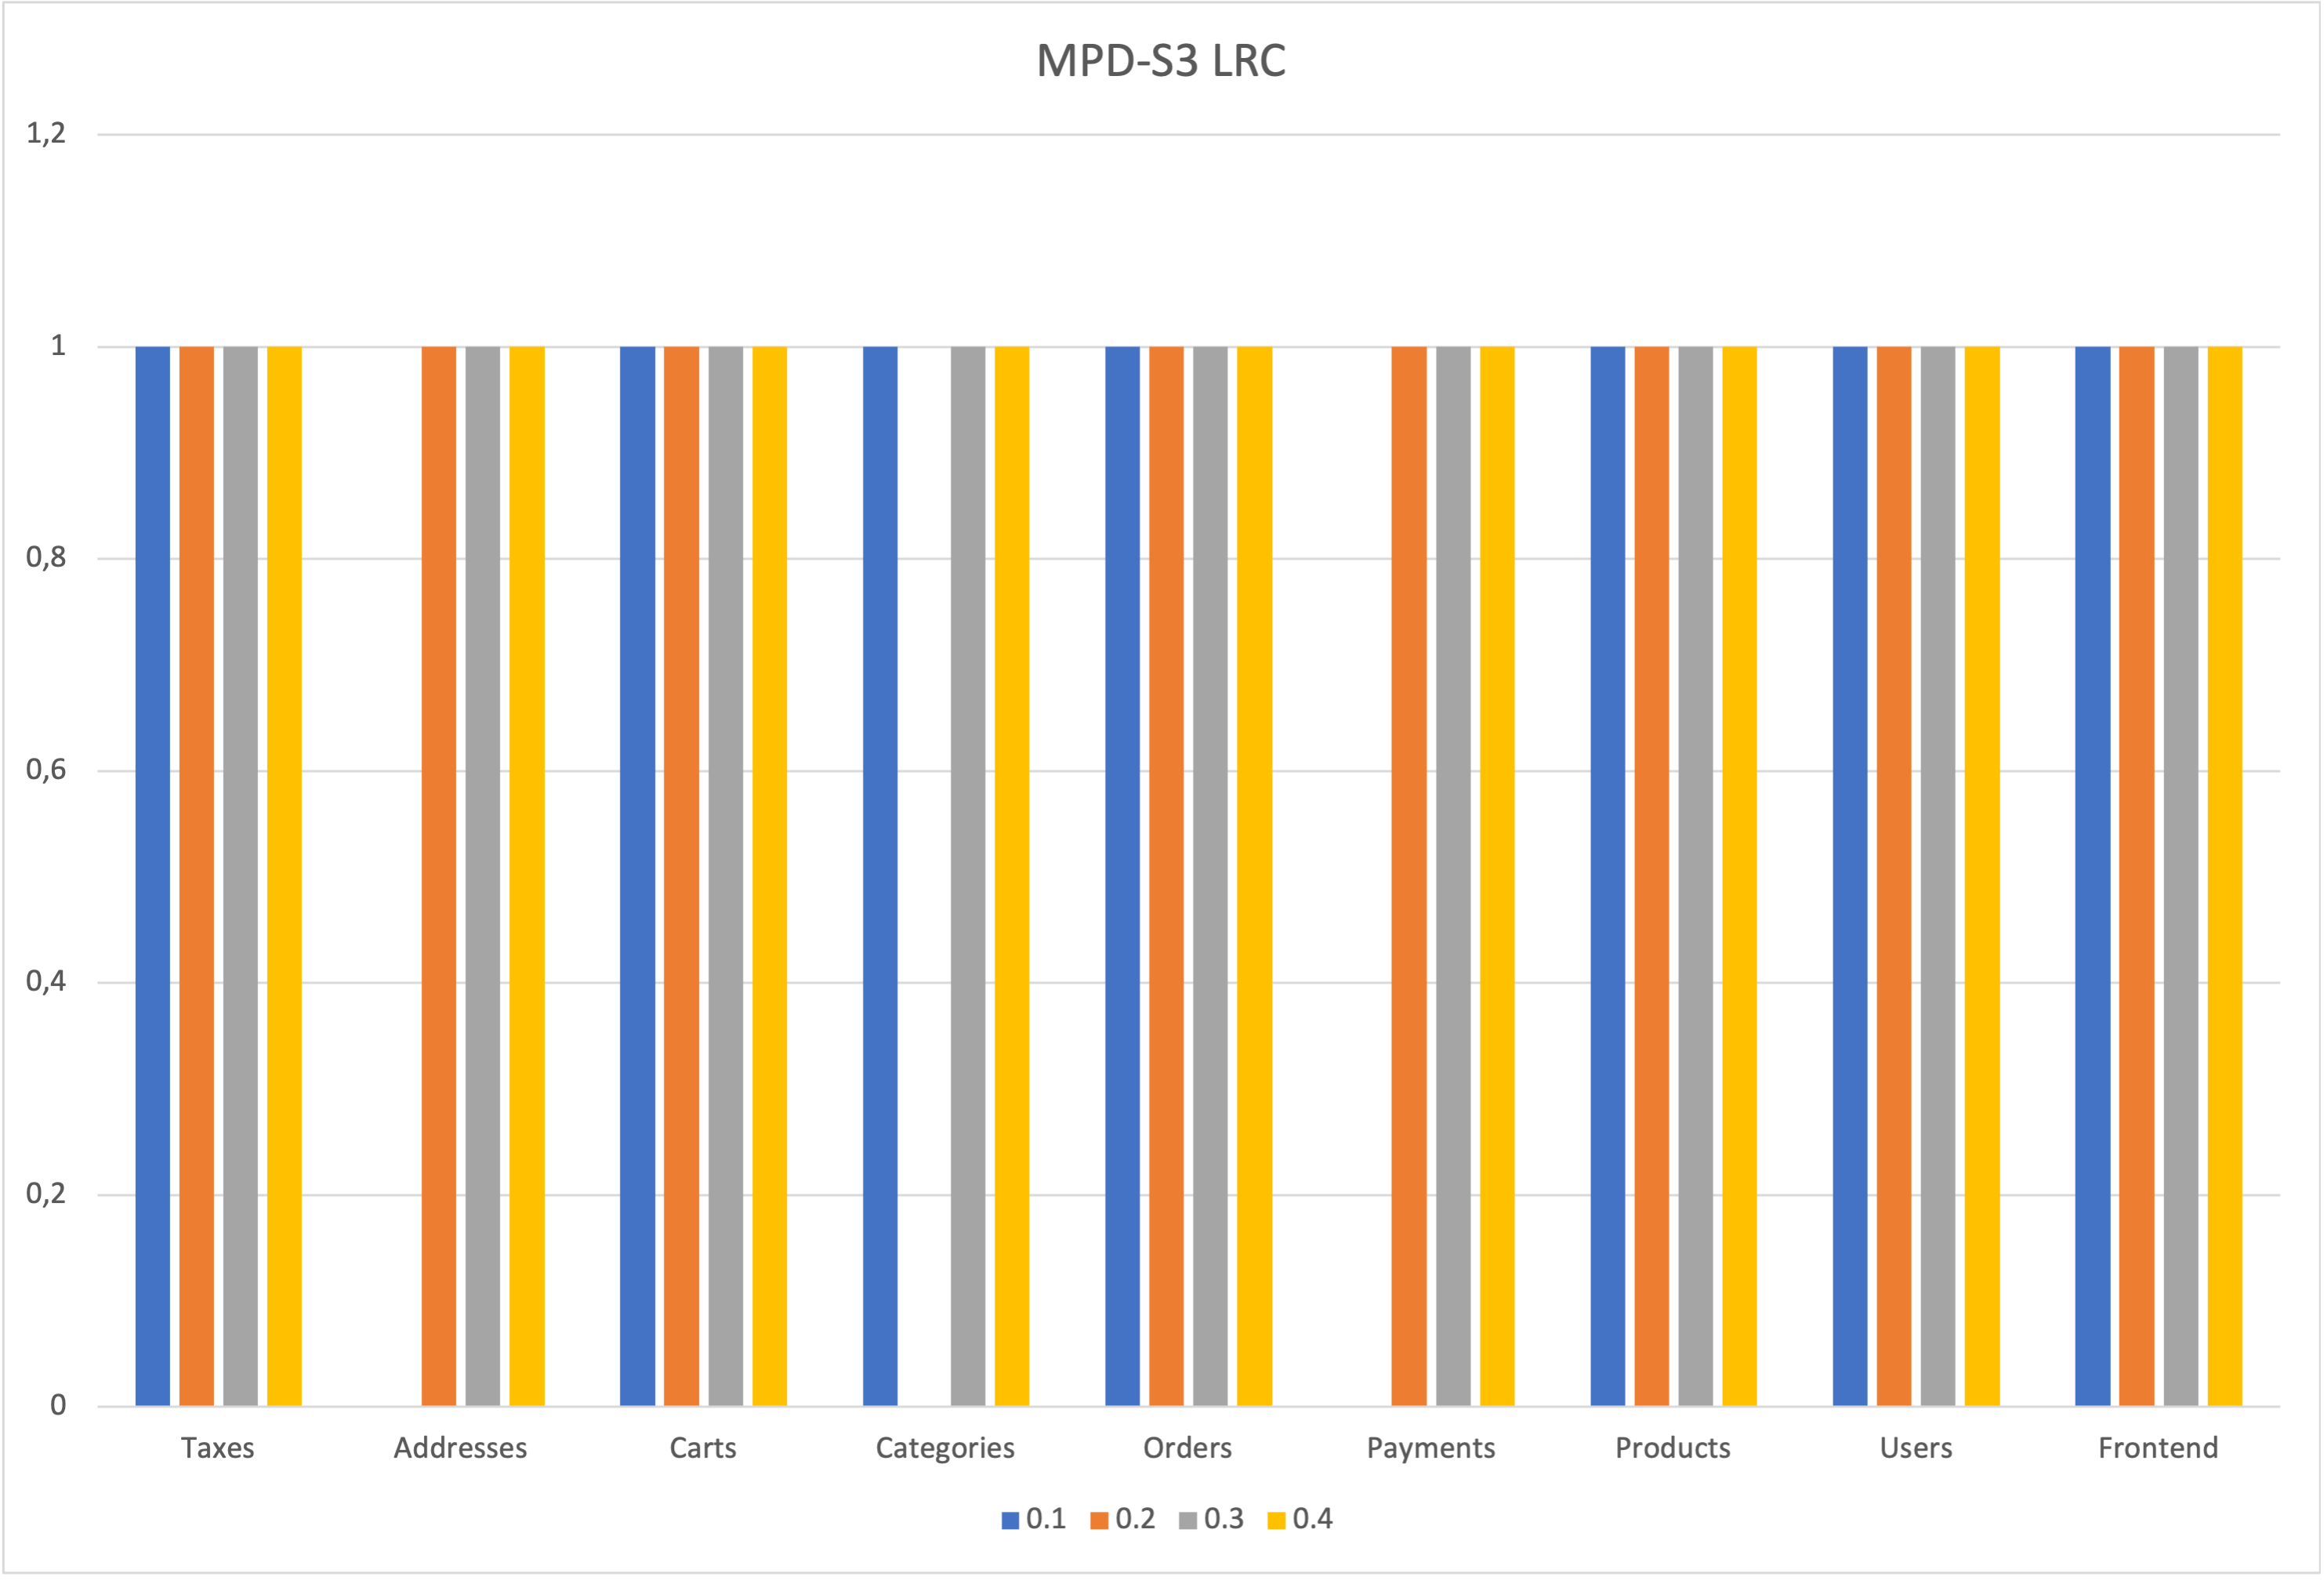
\includegraphics[scale=0.50]{res/images/ra/ra_lrc.png}
        \caption{Grafico metrica MPD-S3 LRC}
    \end{figure}
    \begin{center}
        \rowcolors{2}{white}{blue!20}
    \end{center}
\end{center}

\begin{center}
    \textbf{MPD-S4 CODCO} \\
    Grafo relativo ai valori della metrica relativa alla code coverage con valori espressi in percentuale, come evidenziato nel 
        grafico il dato minimo desiderabile previsto dalle \dext{NormeDiProgetto\_4.0.0} è superiore ad 80
        \begin{figure}[!htb]
        \centering
        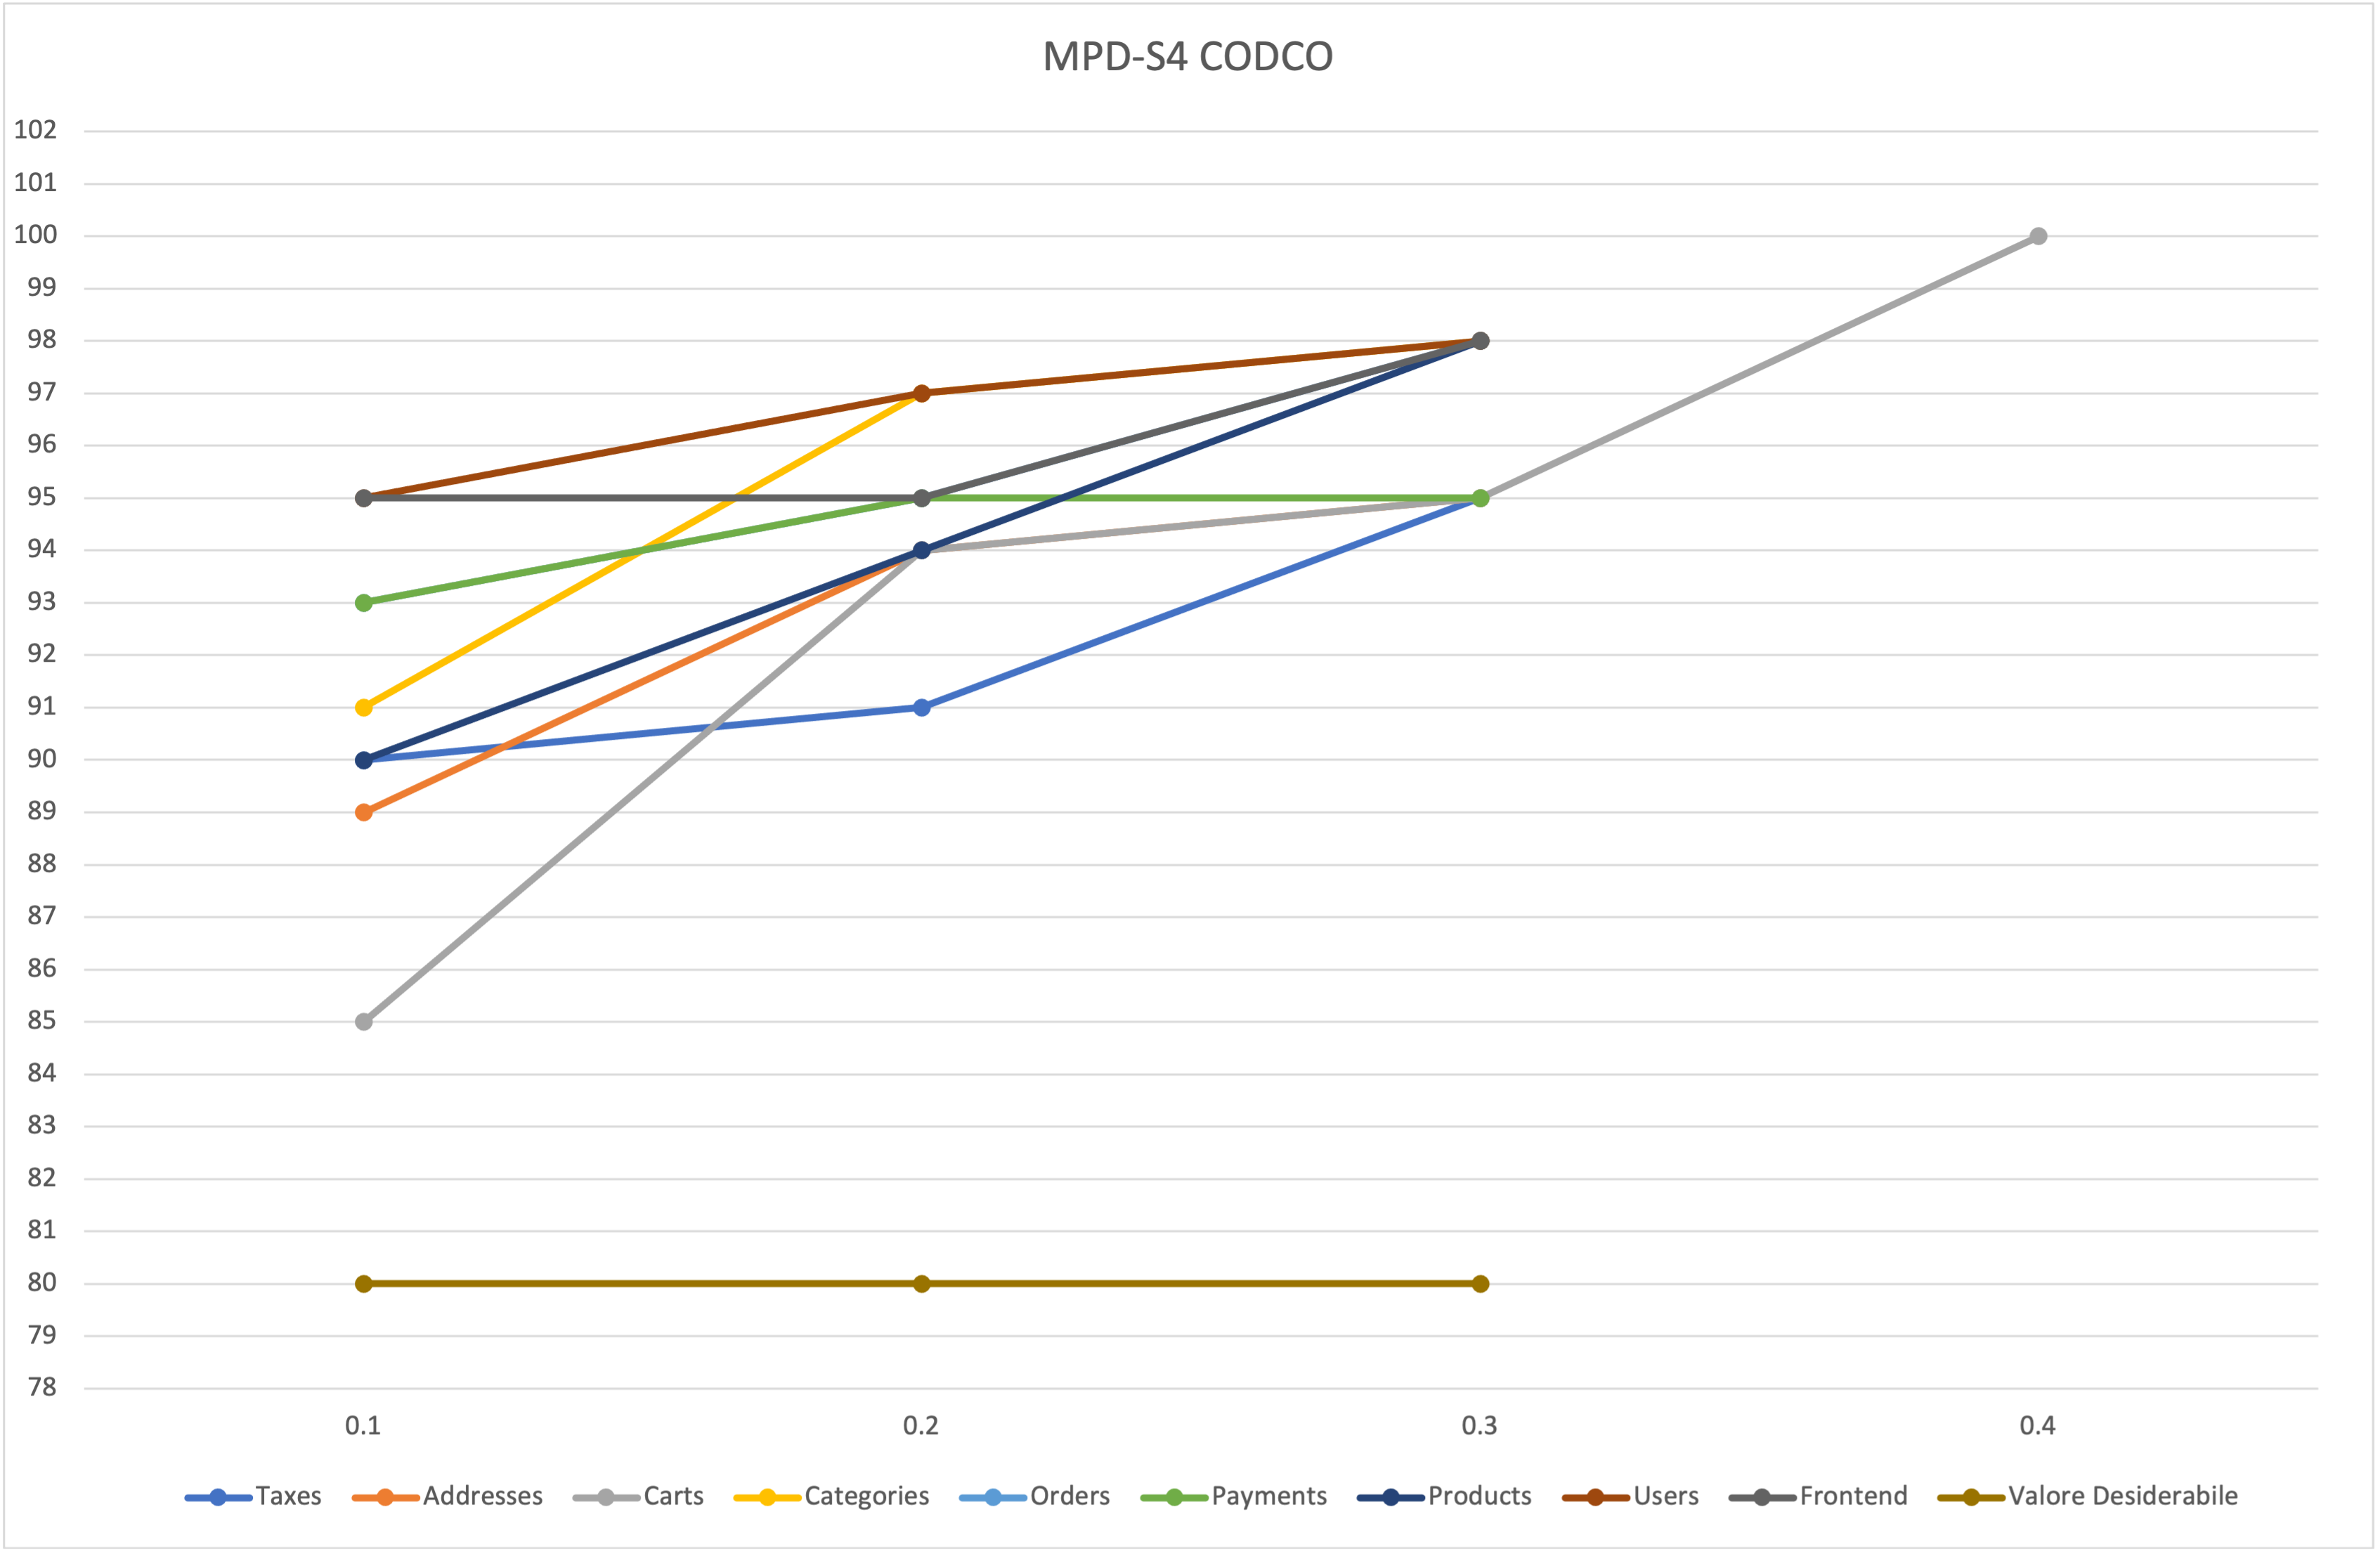
\includegraphics[scale=0.50]{res/images/ra/ra_codco.png}
        \caption{Grafico metrica MPD-S4 CODCO}
    \end{figure}
    \begin{center}
        \rowcolors{2}{white}{blue!20}
    \end{center}
\end{center}

\newpage
\paragraph{MPR-6: Requisiti obbligatori soddisfatti (PROS)}\label{_SV}
Di seguito sono presentanti i dati relativi ai requisiti obbligatori soddisfatti è trascurabile una rappresentazione grafica dei requisti obbligatori di 
qualità e vincolo in quanto soddisfatti sin dall'avvio dell'attività di progetto.

\begin{center}
        \begin{figure}[!htb]
        \centering
        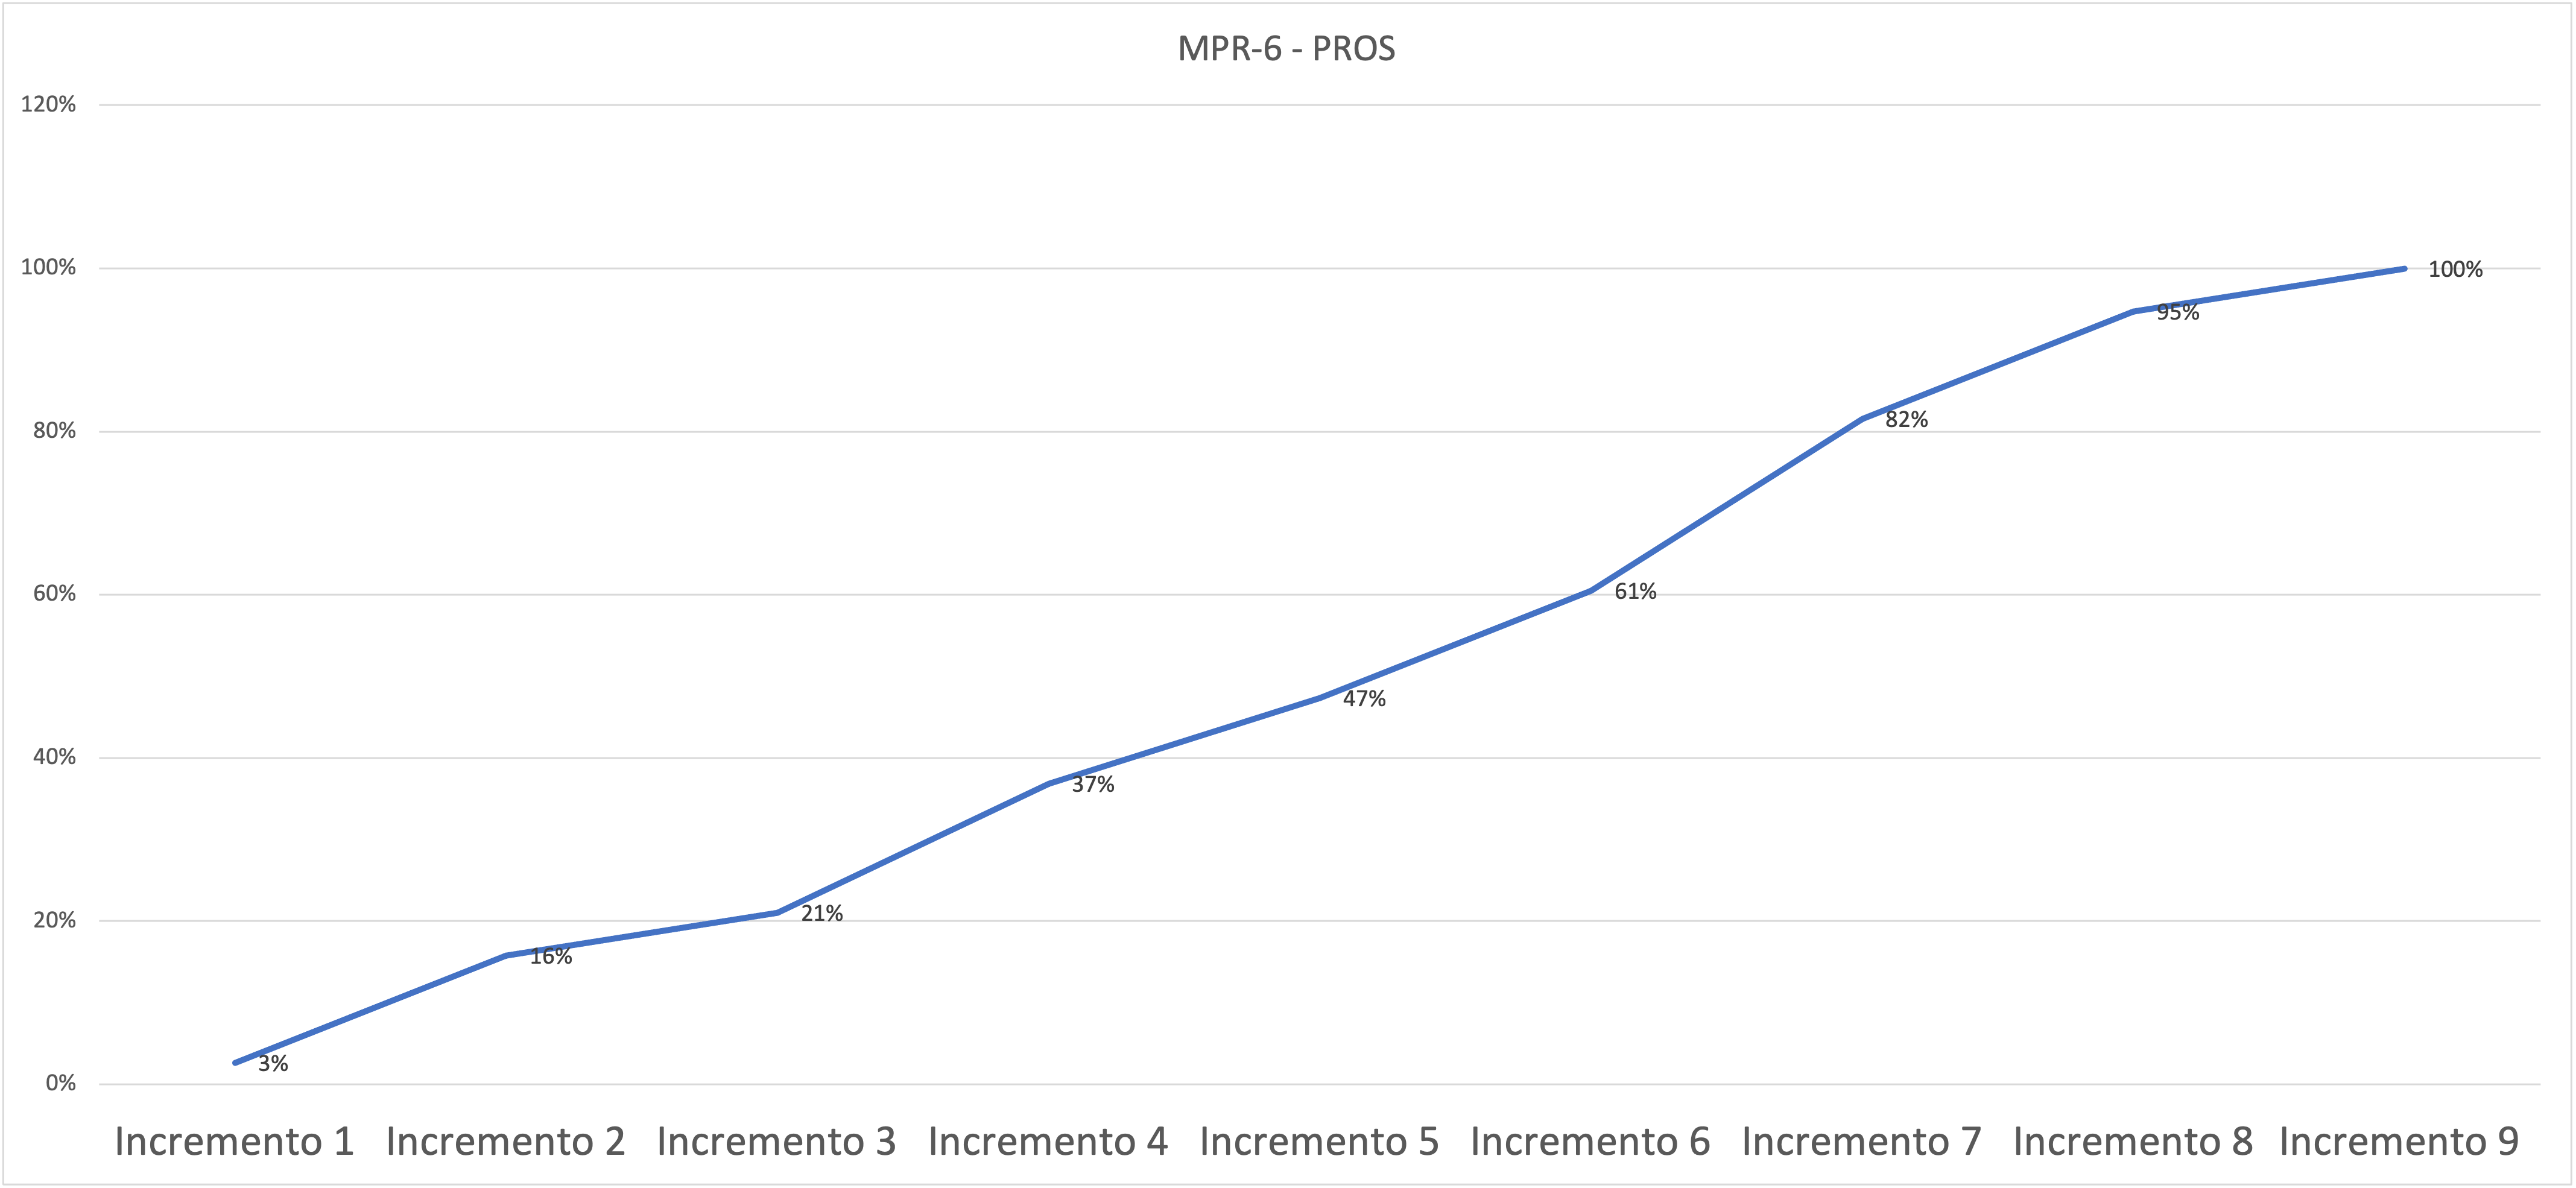
\includegraphics[scale=0.40]{res/images/ra/RA_PROS.png}
        \caption{Grafico metrica MPR-6 PROS}
    \end{figure}
    \begin{center}
        \rowcolors{2}{white}{blue!20}
    \end{center}
\end{center}

\begin{center}
    \rowcolors{2}{white}{blue!20}
    \begin{longtable}{|c|c|c|c|c|}
        \hline
        \rowcolor{lighter-grayer}
        \textbf {Tipo Requisiti} & \textbf{Requisiti Obbligatori Individuati} & \textbf{Soddisfatti} & \textbf{Percentuale} & \textbf{Esito} \\
        \hline
        \endfirsthead

        \hline
        Funzionali & 38 & 31 & 82 \%  & non accettabile                \\
        Qualità & 4 & 4 & 100 \% & accettabile                         \\
        Vincolo & 8 & 8 & 100 \% & accettabile                          \\     
        \hline
        \rowcolor{white}
        \caption{Risultati metrica PROS}
    \end{longtable}
\end{center}


\newpage

\paragraph{MPR-7: Requisiti opzionali non soddisfatti (RONS)}\label{_SV}

\begin{center}
        \begin{figure}[!htb]
        \centering
        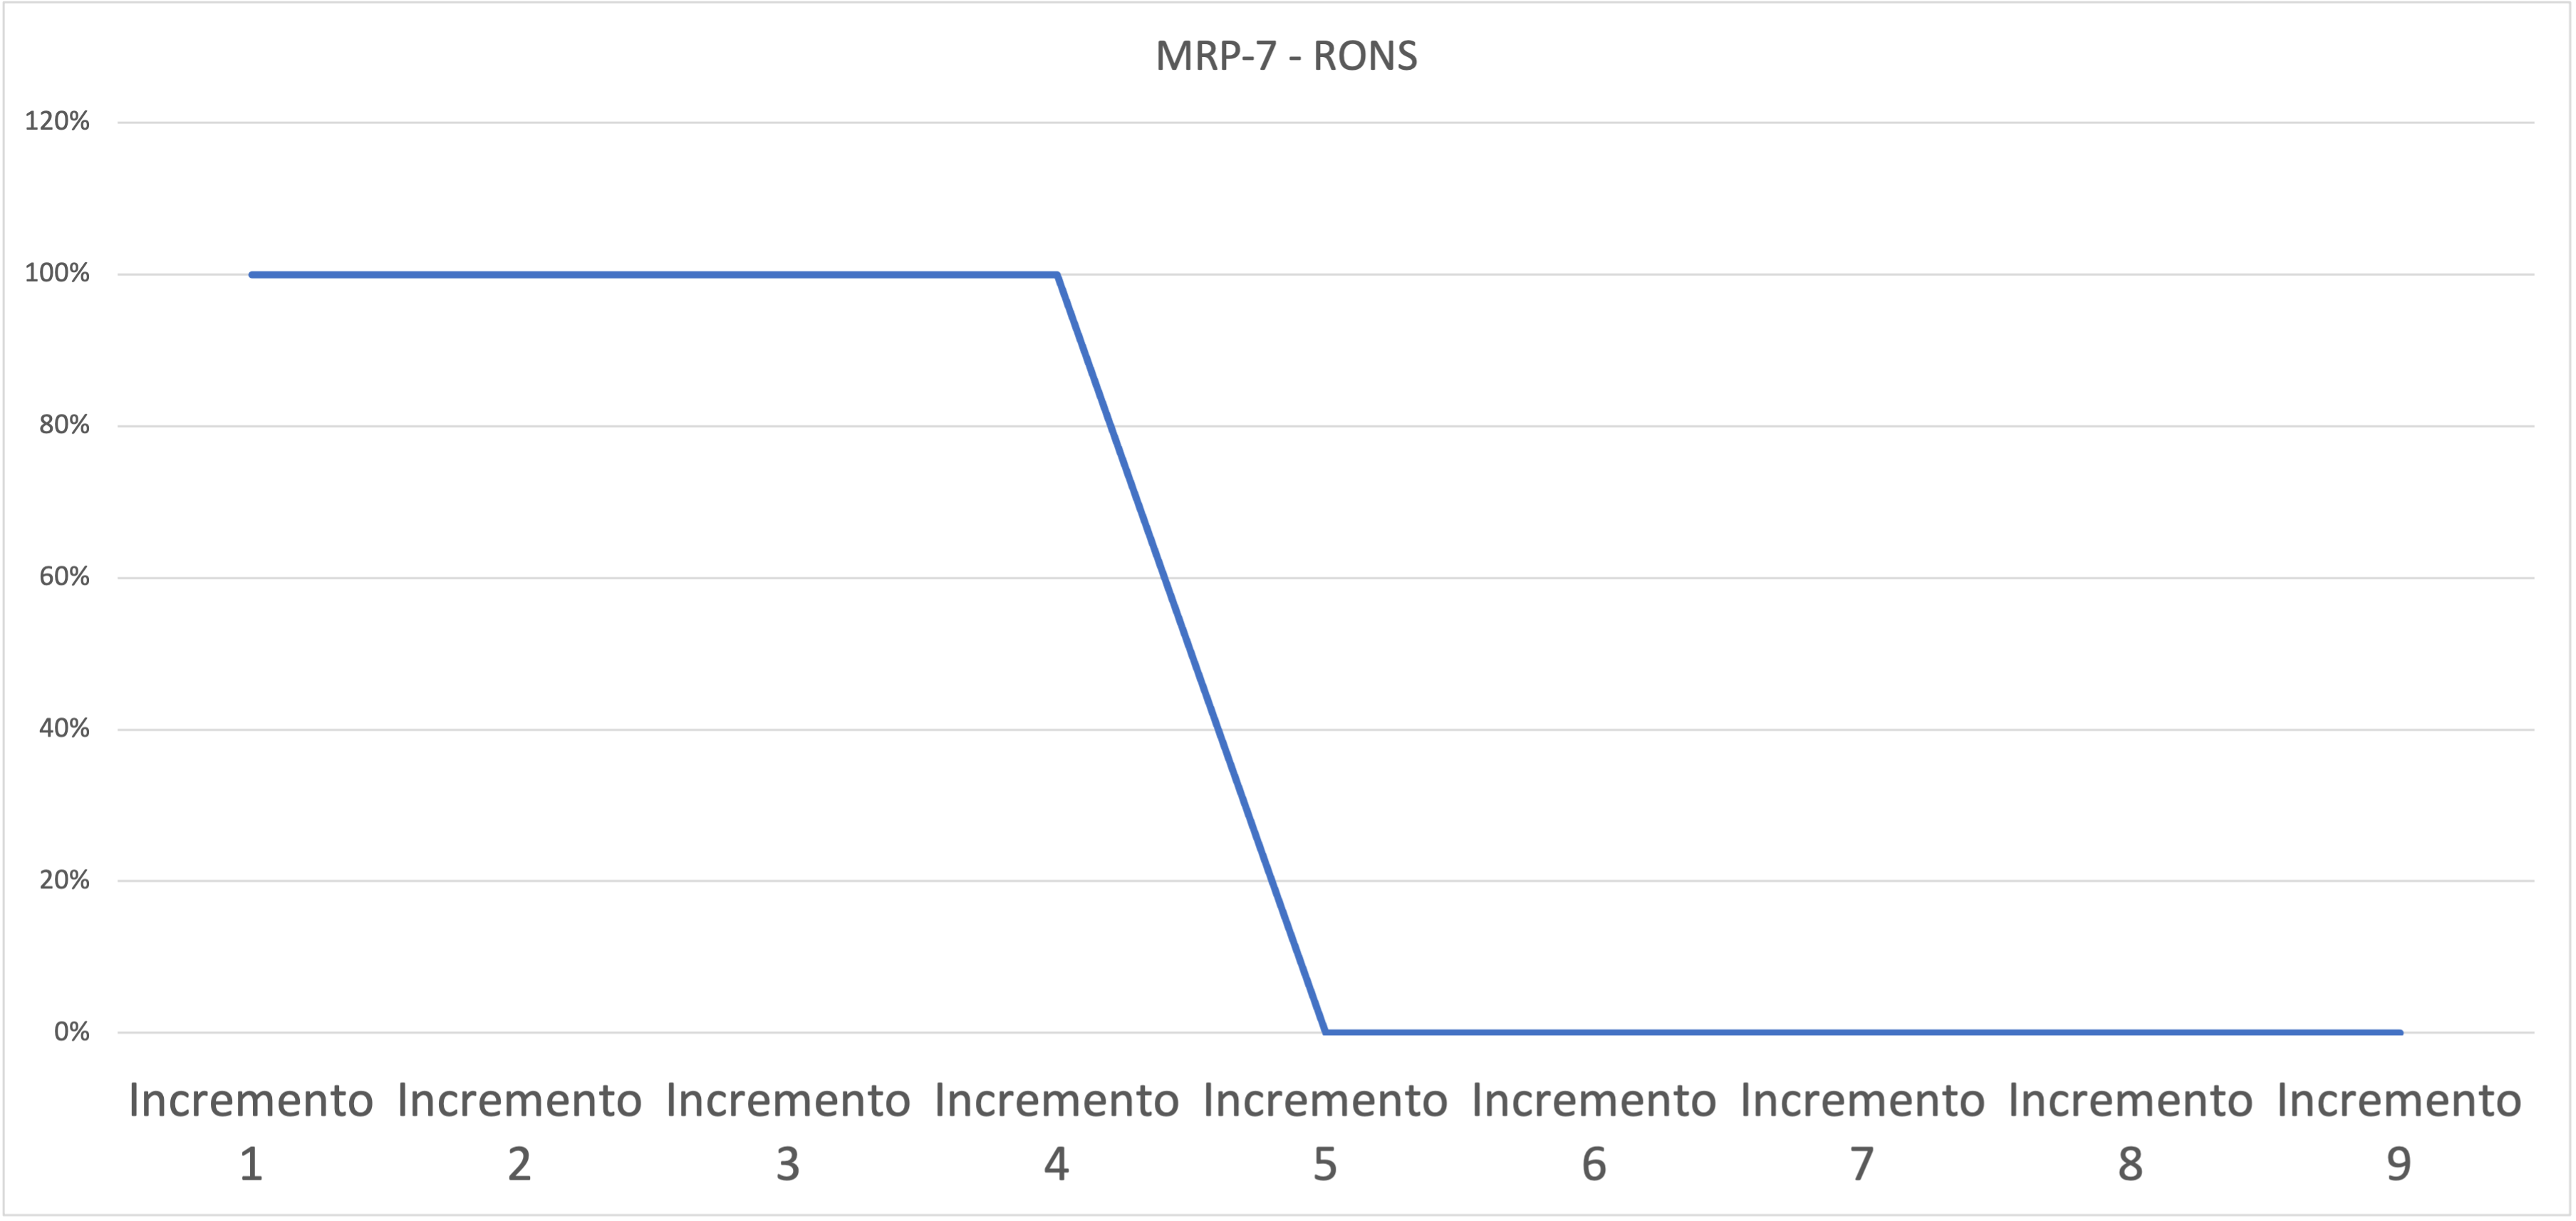
\includegraphics[scale=0.40]{res/images/ra/RA_RONS.png}
        \caption{Grafico metrica MPR-7 RONS}
    \end{figure}
    \begin{center}
        \rowcolors{2}{white}{blue!20}
    \end{center}
\end{center}

\begin{center}
    \rowcolors{2}{white}{blue!20}
    \begin{longtable}{|c|c|c|c|c|}
        \hline
        \rowcolor{lighter-grayer}
        \textbf {Tipo Requisiti} & \textbf{Requisiti Opzionali Individuati} & \textbf{Non Soddisfatti} & \textbf{Percentuale} & \textbf{Esito} \\        \hline
        \endfirsthead

        \hline
        Funzionali & 1 & 0 & 0 \%  &  accettabile        \\
        Qualità & 0 &  &  &                        \\
        Vincolo & 0 & & &                        \\  
        \hline
        \rowcolor{white}
        \caption{Risultati metrica RONS}
    \end{longtable}
\end{center}


\newpage
\paragraph{MPR-8: Requisiti opzionali non soddisfatti (RDNS)}\label{_SV}

\begin{center}
        \begin{figure}[!htb]
        \centering
        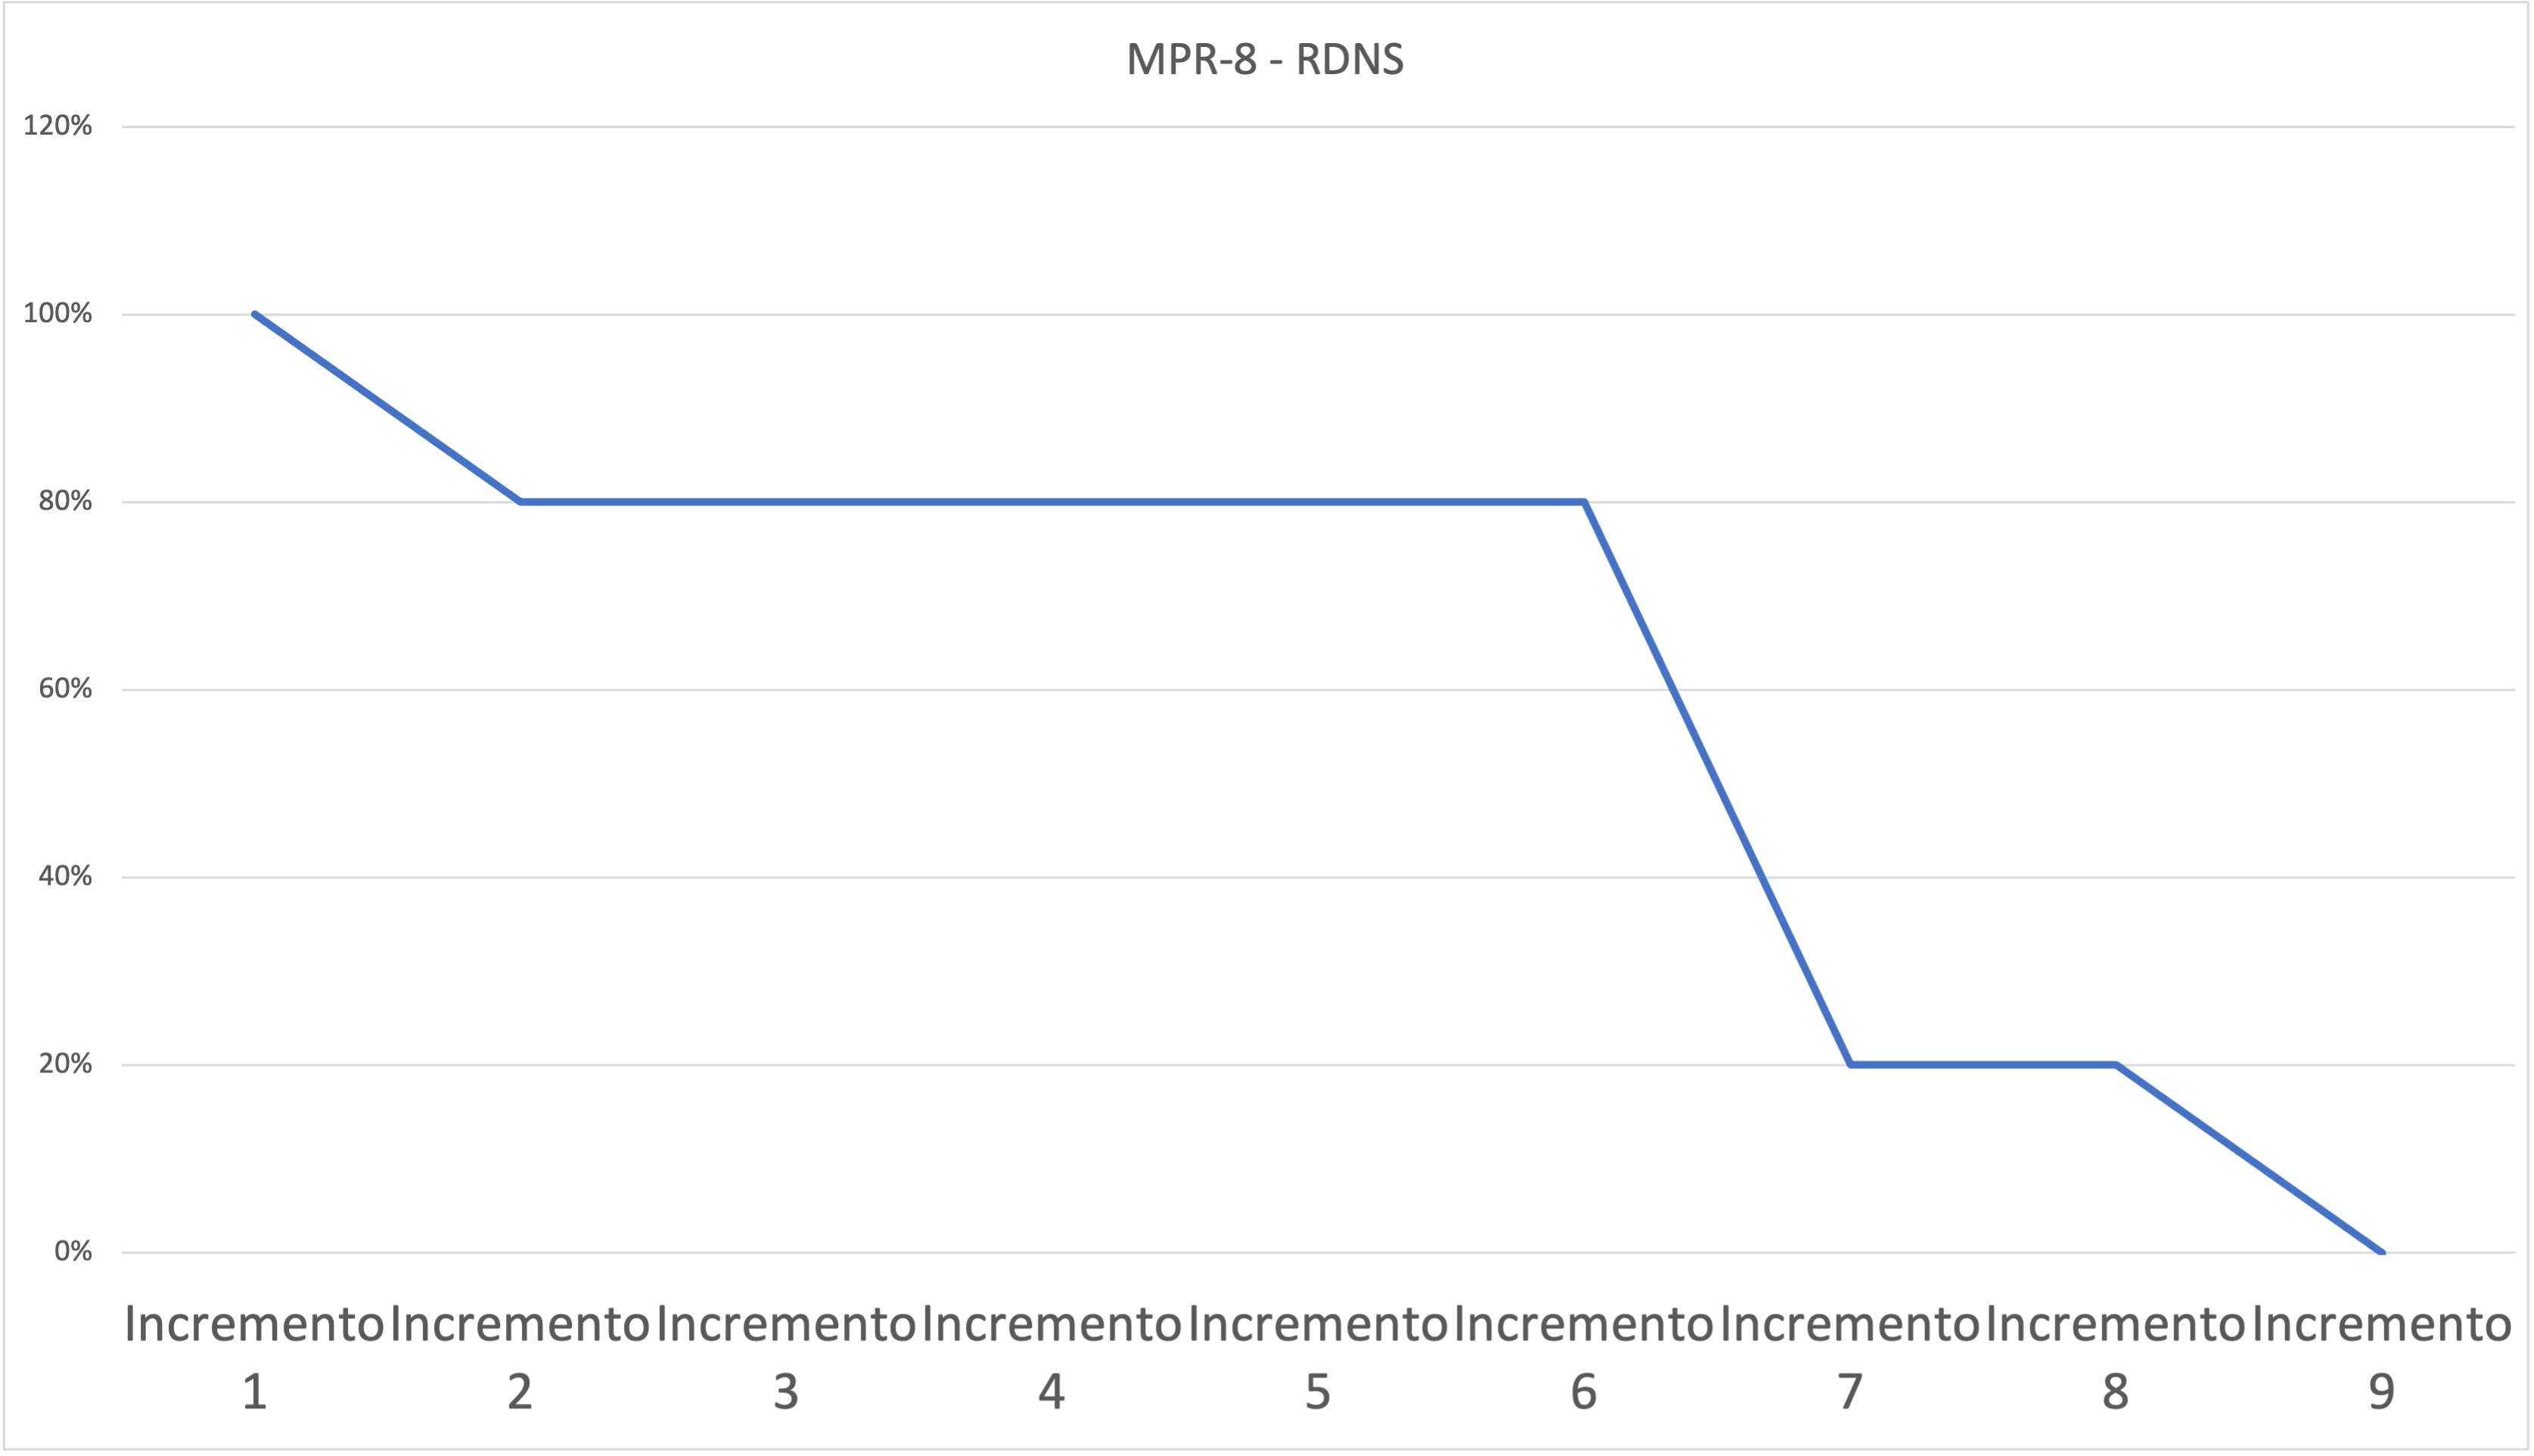
\includegraphics[scale=0.40]{res/images/ra/RA_RDNS_FUNZ.png}
        \caption{Risultati metrica RDNS dei requisiti di funzionalità per periodo}
    \end{figure}
    \begin{figure}[!htb]
        \centering
        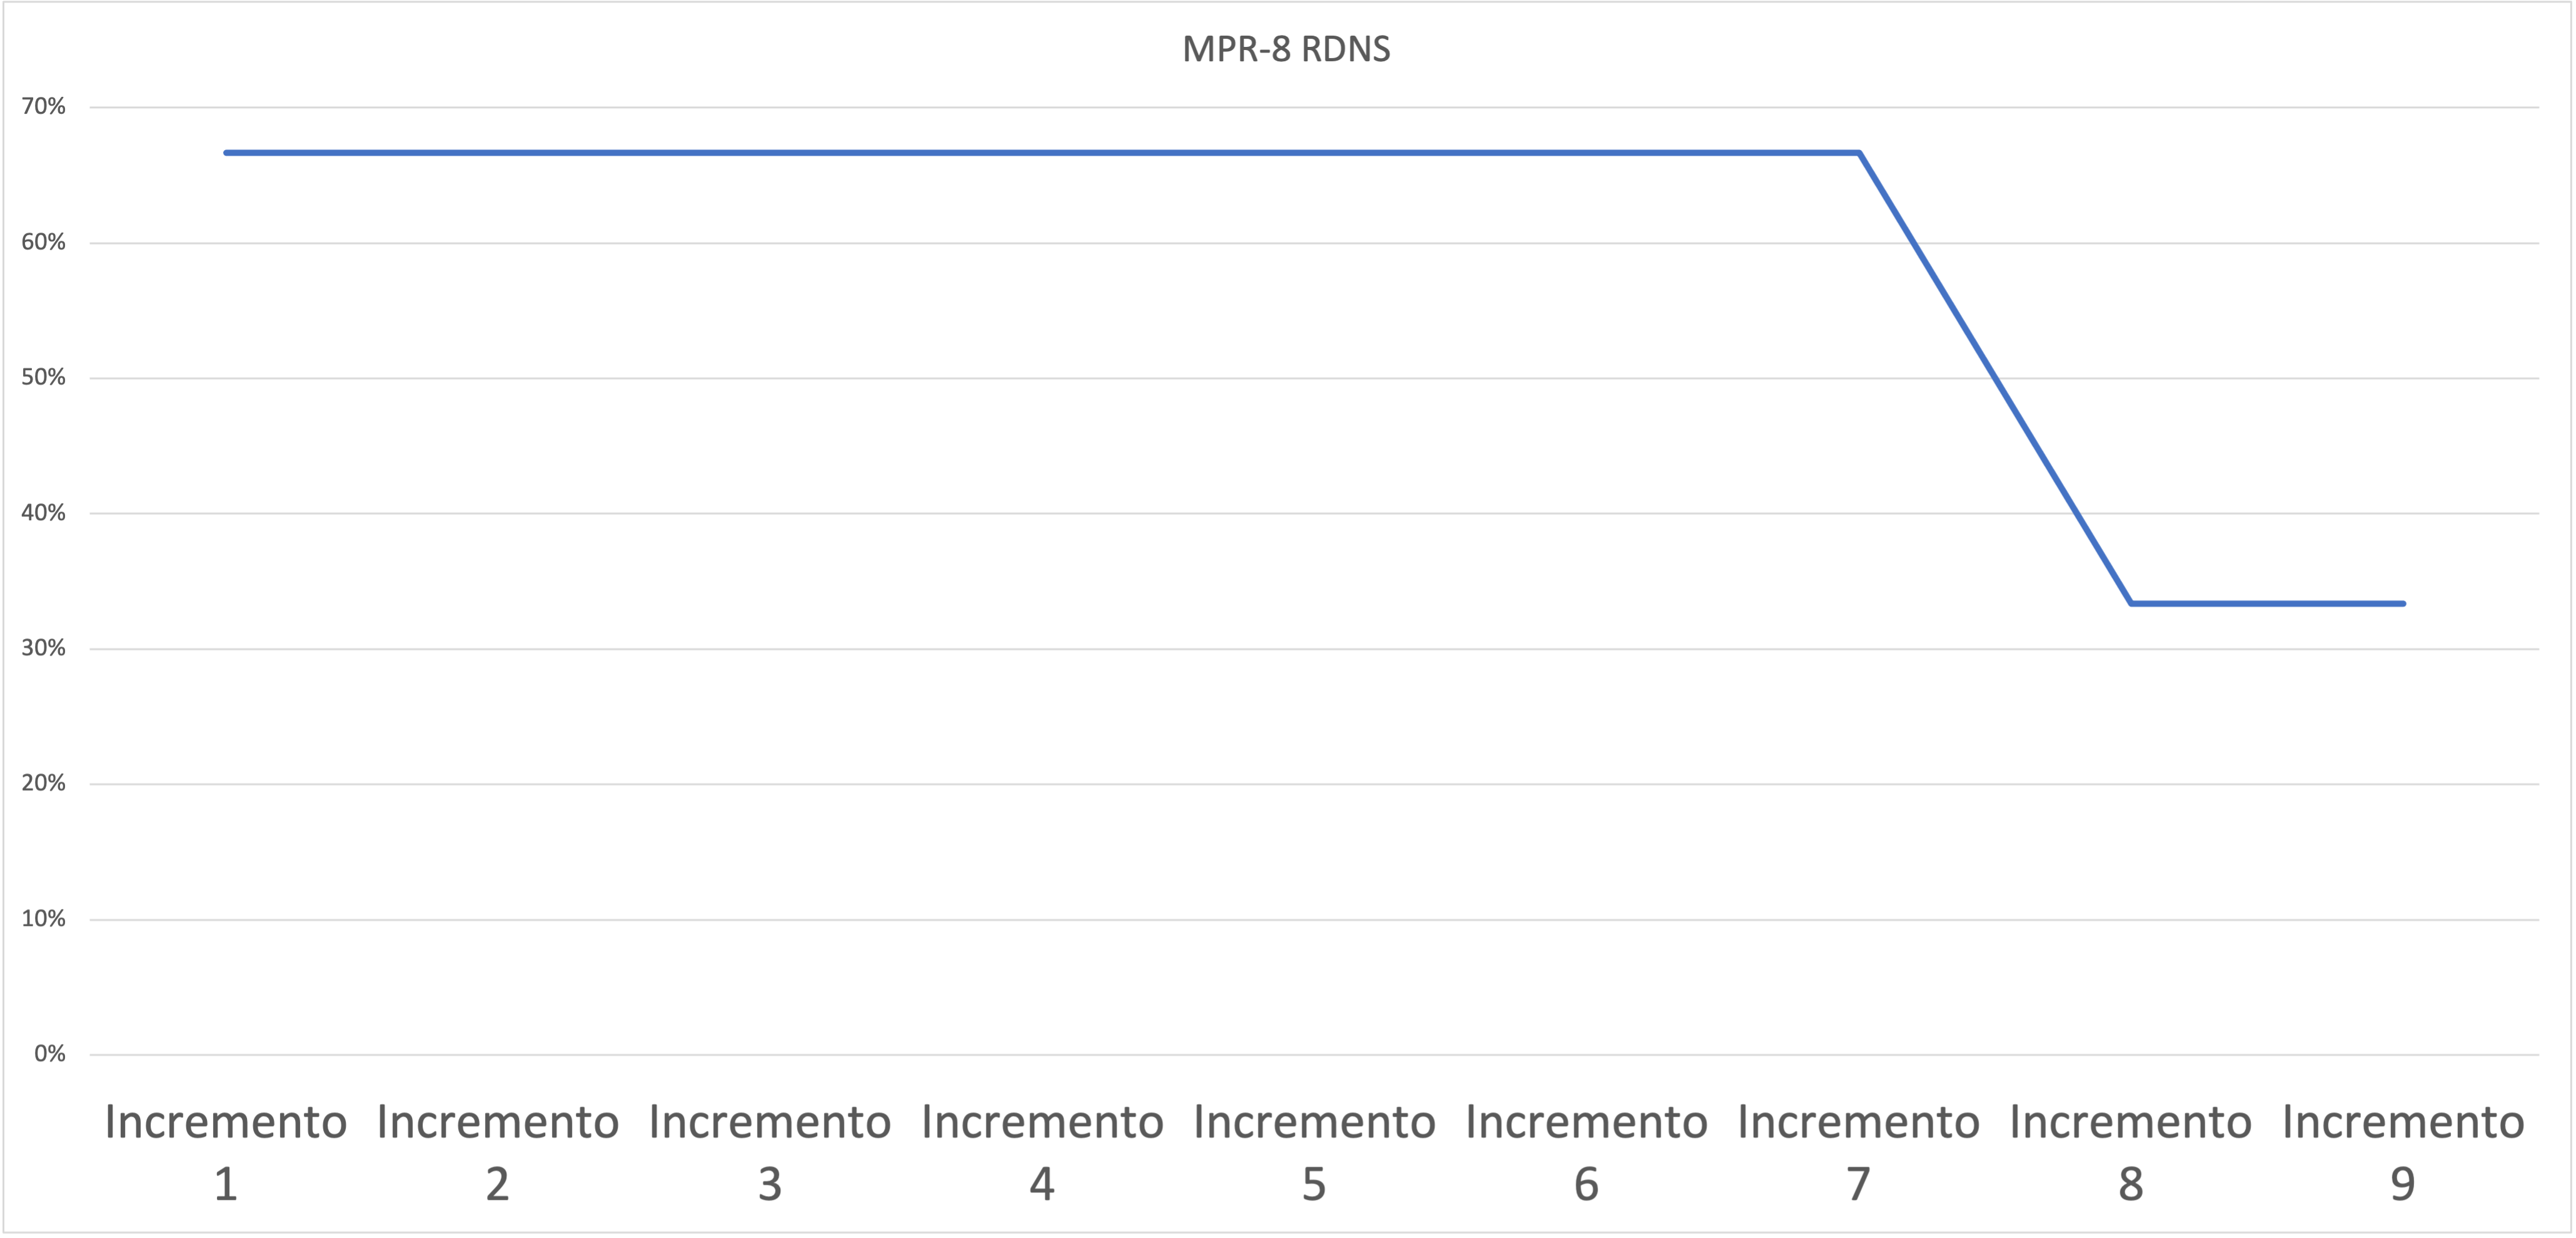
\includegraphics[scale=0.40]{res/images/ra/RA_RDNS_VINC.png}
        \caption{Grafico contenente il valore della metrica RDNS dei requisiti di vincolo per periodo}
    \end{figure}
    \begin{center}
        \rowcolors{2}{white}{blue!20}
    \end{center}
\end{center}

\begin{center}
    \rowcolors{2}{white}{blue!20}
    \begin{longtable}{|c|c|c|c|c|}
        \hline
        \rowcolor{lighter-grayer}
        \textbf {Tipo Requisiti} & \textbf{Requisiti Desiderabili Individuati} & \textbf{Non Soddisfatti} & \textbf{Percentuale} & \textbf{Esito} \\ \hline
        \endfirsthead

        \hline
        Funzionali & 5 & 1 & 20 \%  &  accettabile                \\
           Qualità & 0 &  &  &                        \\
           Vincolo & 3 &  2 &  67 \%&    accettabile                    \\ 
        \hline
        \rowcolor{white}
        \caption{Risultati metrica RDNS}
    \end{longtable}
\end{center}